% !TeX root = ../main.tex

\chapter{概要设计}
在第二章中介绍了一些经典的分布式存储系统,第三章介绍了本系统的需求分析,本论文试图从已有的对象存储系统方案出发,结合系统的实际需求,将原有方案改进优化,构建设计分布式对象存储系统。本章将会从整体出发,阐述本对象存储系统的设计思路,首先将会介绍系统的整体架构,在整体架构之上,将会介绍系统中每个模块的概要设计,包括四个功能模块的概要设计、对象数据存储模块的概要设计和元数据模块的概要设计,为后续介绍模块的详细实现做铺垫。

\section{系统整体架构}%4.1
为了提升系统的可用性和可扩展性,系统选择了分层的架构进行设计。系统的逻辑架构图如图4.1所示,主要分为访问层、接入层、业务层和存储层四个层次。

\begin{figure}[h]
  \centering
  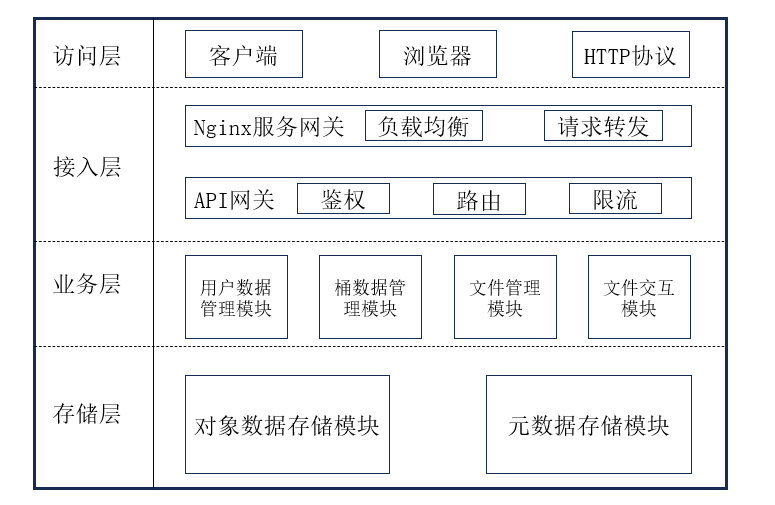
\includegraphics[width=0.9\textwidth]{系统架构图.png}
  \caption{系统逻辑架构图}
\end{figure}

访问层是用户访问系统的媒介,用户可以用客户端或浏览器等媒介来访问系统,也可以直接向系统发送HTTP请求来访问系统。

接入层主要负责对用户发来的请求做权限验证,系统使用Ngnix作为服务网关,对于鉴权通过的请求,接入层会根据负载均衡策略将请求转发到对应的应用服务上。API网关负责路由转发,限流,熔断等,是所有对外接口的总入口。所有的外部请求都会先经过API网关,再由API网关进行转发。

业务层包含了基于微服务思想拆分的不同的服务模块,包括用户数据管理模块,桶数据管理模块,文件管理模块和文件交互模块,不同的服务模块负责不同的功能。为了提升系统的可用性,这些服务模块进行了冗余部署,当某模块的节点出现故障无法访问时,API网关会将请求转发到其他模块,继续为用户提供服务。

存储层包含两个部分,一个是元数据存储模块,一个是对象数据存储模块。元数据存储模块使用MongoDB实现,负责保存系统中的元数据。对象数据存储模块则是本系统自主开发实现的,负责保存系统中具体的对象数据,这个模块的设计与实现将在后文进行展开。

\section{功能模块设计}
本系统的业务层中,主要有用户数据管理模块、桶数据管理模块、文件管理模块和文件交互模块这四个业务功能模块。我们对每一个模块的功能进行继续细分,可以得到图4.2,该图展示了详细的业务功能模块的功能划分。

\begin{figure}[h]
  \centering
  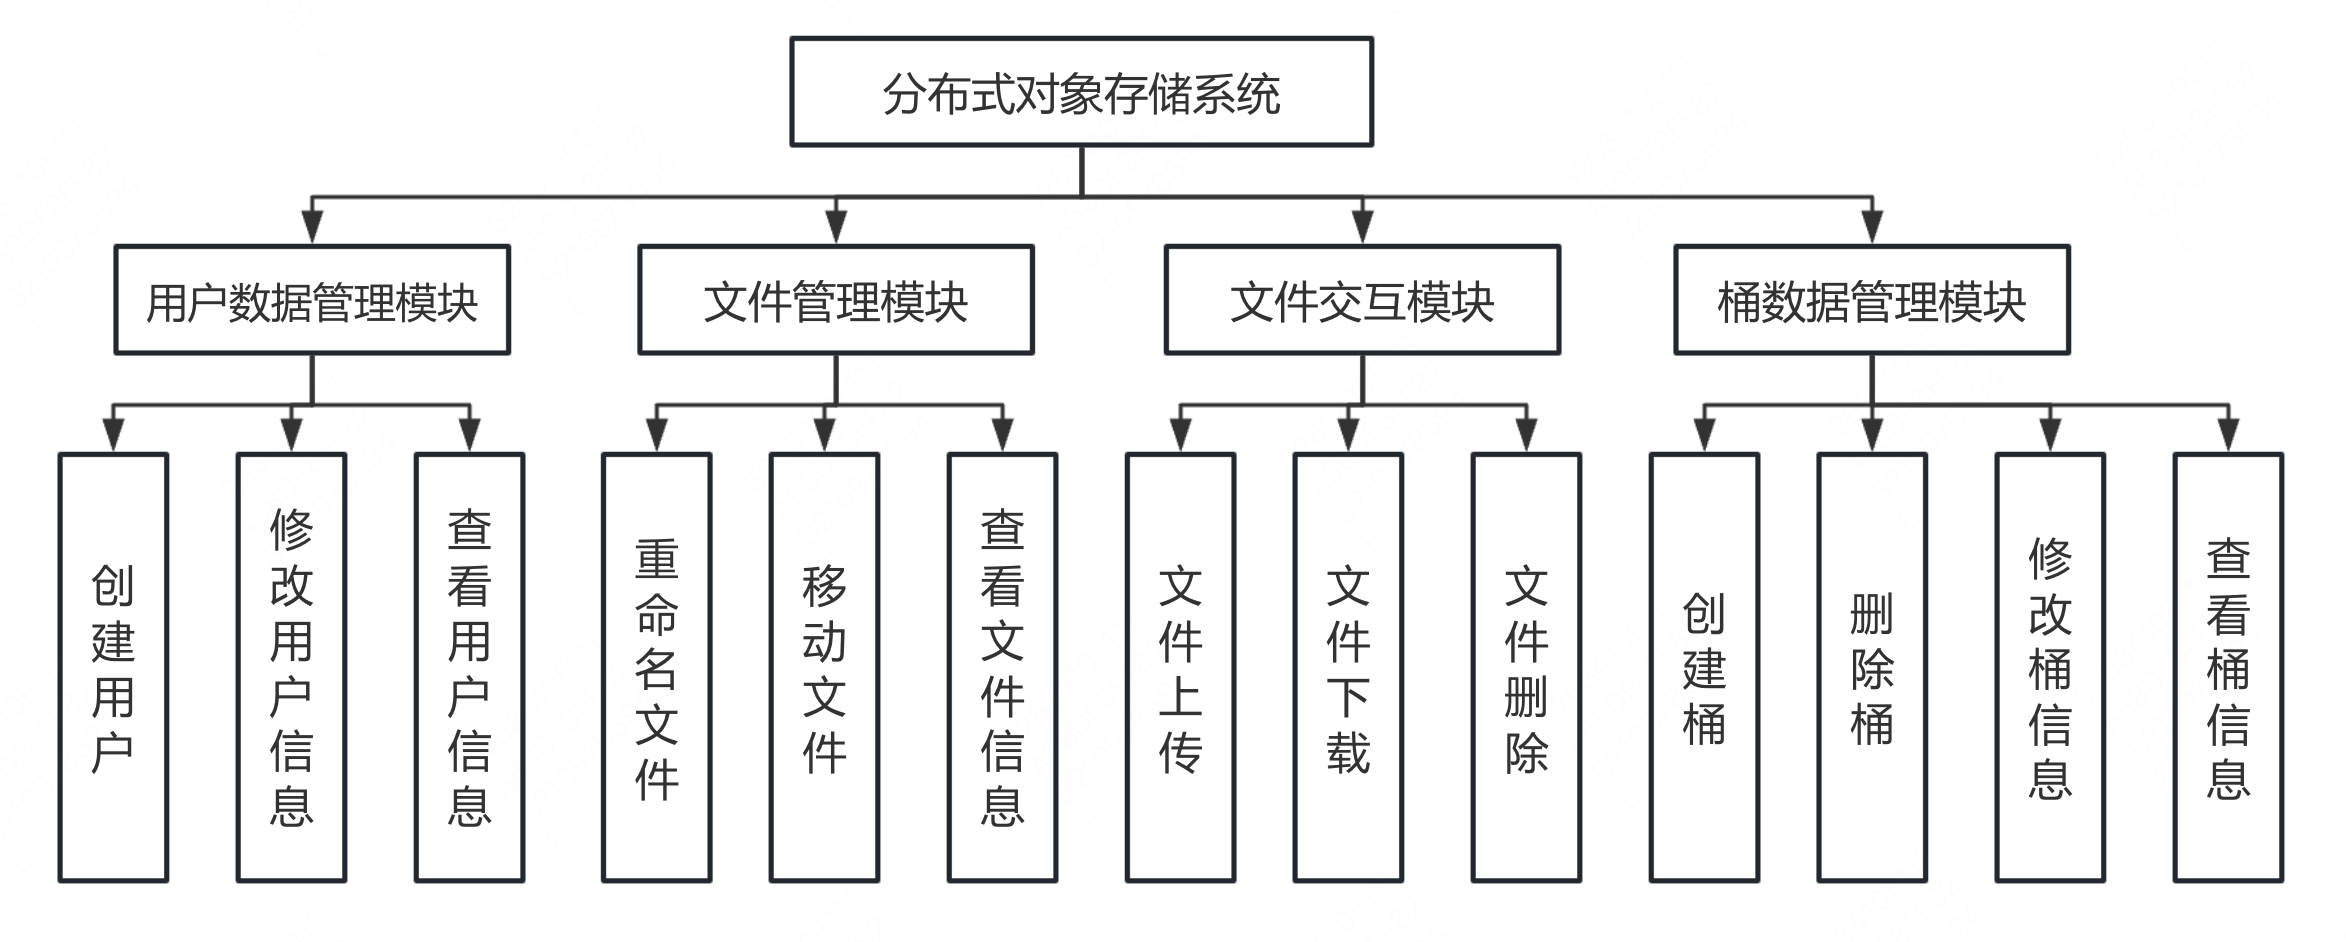
\includegraphics[width=1.0\textwidth]{功能模块图.png}
  \caption{系统功能模块图}
\end{figure}

\subsection{用户数据管理模块概要设计}

用户数据管理模块有创建用户、修改用户信息和查看用户信息三个功能。该模块的活动图如图4.3所示。

在整个流程的起点,用户会向系统发起操作请求,网关在接收到请求后会将请求路由到用户数据管理模块中。模块会先判断请求是否是创建用户请求,如果是的话,再会判断用户需要创建的用户名是否已经在系统中存在,如果不存在同名用户则将按照用户输入的信息创建新用户,反之则将向用户返回系统中已有同名用户;如果不是创建用户请求,模块则会先判断此请求是否通过鉴权,如果没有通过鉴权则会返回请先登录鉴权的提示,对于通过鉴权的操作,则进行对应的业务处理,并将处理的结果进行返回。

\begin{figure}[h]
  \centering
  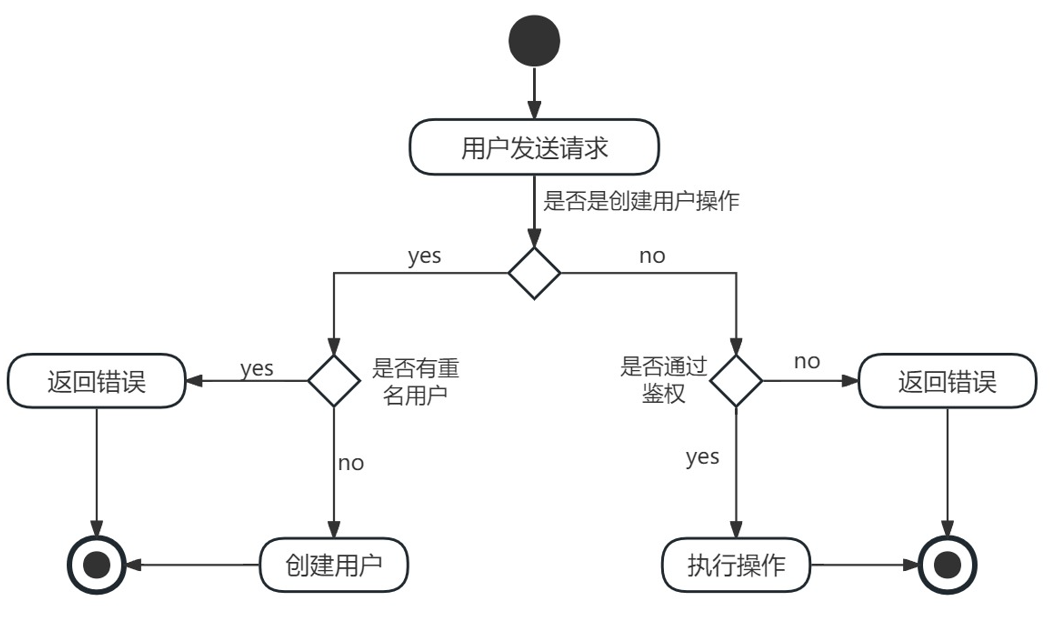
\includegraphics[width=0.78\textwidth]{用户管理活动图.png}
  \caption{用户管理活动图}
\end{figure}

\subsection{桶数据管理模块概要设计}
桶数据管理模块主要有创建桶、删除桶、修改桶信息和查看桶信息四个功能。该模块的活动图如图4.4所示。

\begin{figure}[h]
  \centering
  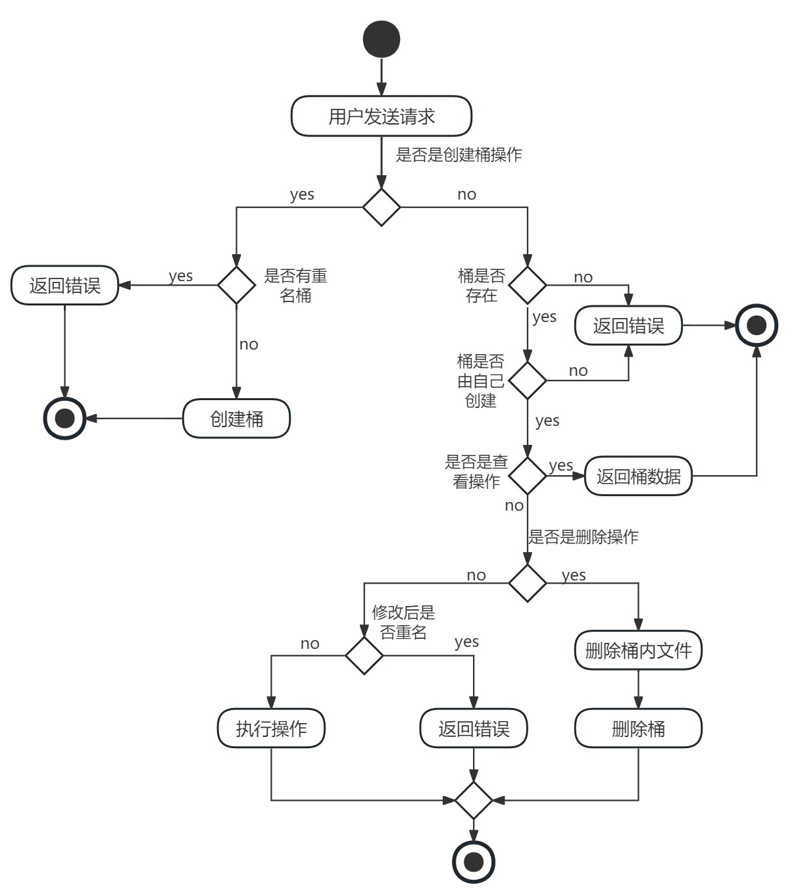
\includegraphics[width=0.70\textwidth]{桶数据管理活动图.png}
  \caption{桶数据管理活动图}
\end{figure}

模块在接收到用户的请求后,首先会判断此操作是否是创建桶操作,如果是的话则会检查要创建的桶是否已经有同名的桶存在,有则返回创建失败,反之则返回创建成功;如果不是创建桶操作,模块会先判断请求操作的桶是否存在且由用户创建,验证通过后会执行对应的业务逻辑,如果是查看桶信息操作则将返回对应的数据,如果是删除桶操作则会将桶内文件进行清空,如果是修改桶信息操作则会检查修改后是否会出现重名的桶,如果出现则不允许这次修改桶信息的请求。

本模块还提供了查看创建的全部桶的功能,这个功能只需要在鉴权通过后获取用户的uid,然后根据uid返回此用户创建的全部桶信息即可。
\subsection{文件管理模块概要设计}
文件管理模块主要有重命名文件、移动文件和查看文件信息三个功能。该模块的活动图如图4.5所示。

\begin{figure}[h]
  \centering
  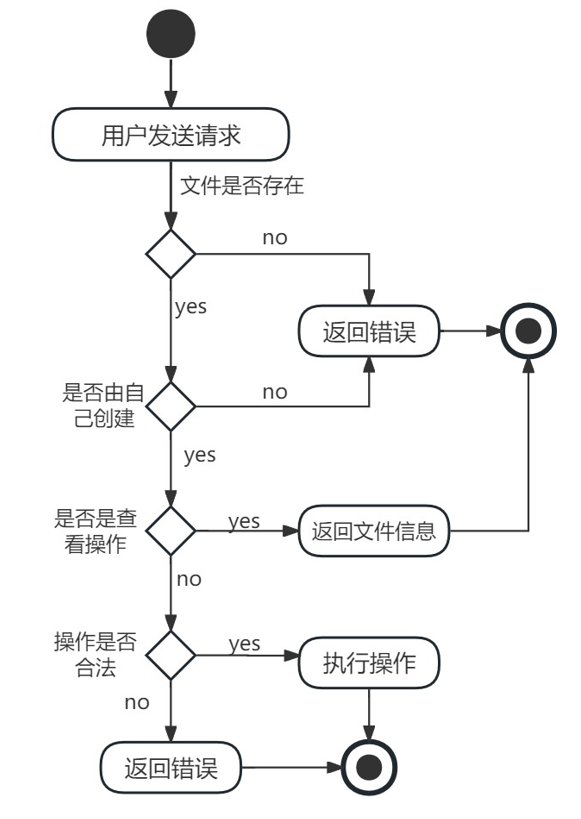
\includegraphics[width=0.45\textwidth]{文件管理活动图.png}
  \caption{文件管理活动图}
\end{figure}

模块在接收到用户的请求后,首先会判断此操作提供的文件是否存在且为用户创建的,如果不是的话则将向用户返回错误信息,然后会判断是否是查看文件信息操作,如果是的话则返回对应文件的信息,反之则代表用户需要进行重命名或移动文件的操作,这时模块会检查操作是否合法,对于重命名文件来说,需要检查操作后是否出现重名文件,对于移动文件来说,不仅需要检查重名的情况,还需要检查目标桶是否存在且由用户创建,如果操作合法则会执行操作,反之返回错误。

本模块还提供了查看桶内全部文件的功能,这个功能在执行前会检查桶是否存在且由用户创建,如果是的话则会将这个桶内的全部文件的信息进行返回,供用户管理。

\subsection{文件交互模块概要设计}
文件交互模块提供文件上传、文件下载、文件删除三个功能。

\begin{figure}[h]
  \centering
  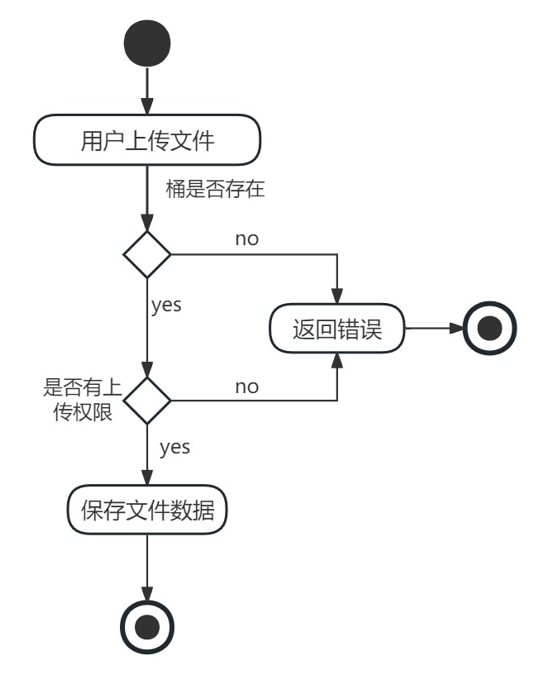
\includegraphics[width=0.42\textwidth]{上传文件活动图.png}
  \caption{文件上传活动图}
\end{figure}

文件上传的活动图如图4.6所示。上传文件时用户需要指定上传至哪个桶,模块会先检查桶是否存在,如果存在还会进一步检查用户是否有上传文件的权限,只有桶的创建者和指定授权过的人才能成功上传文件。

\begin{figure}[h]
  \centering
  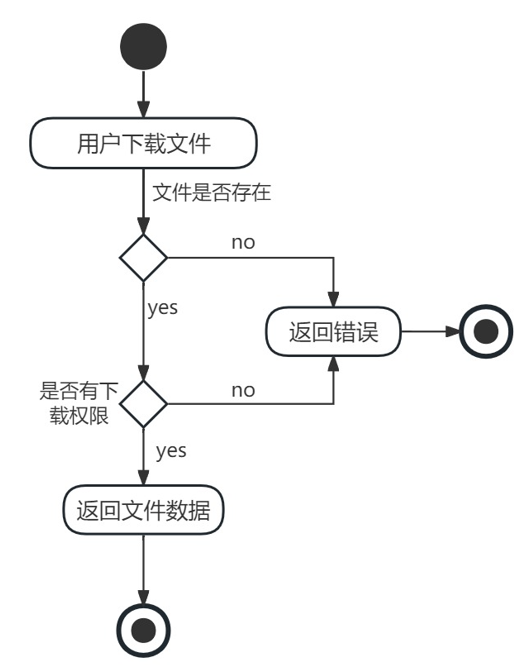
\includegraphics[width=0.42\textwidth]{下载文件活动图.png}
  \caption{文件下载活动图}
\end{figure}

文件下载的活动图如图4.7所示,下载文件时模块会先检查文件是否存在,然后会进一步检查用户是否有权限下载这个文件,如果没有权限则返回错误,有权限则将文件数据返回给用户。

文件删除的流程和文件下载类似,只需要将验证下载权限这一步改为确认文件是由用户创建的即可,因为只有用户的拥有者才可以删除文件。

\section{元数据存储模块设计}
\subsection{元数据数据库选型}
元数据服务是系统的一个核心服务,用户的任何操作都需要和元数据服务交互,元数据维护了用户的所有文件信息,元数据的访问是文件上传和下载的关键环节,因此元数据的数据库对数据存储可靠性和服务可用性要求很高。除此之外,当系统中存储的文件逐渐变多的的时候,元数据的数据量也会逐渐变多,因此元数据数据库也需要有可扩展的特性。另外,元数据数据块中需要保存的内容比较灵活,使用传统的关系型数据库将会难以应对,因此元数据数据库应该选用非结构化的数据库。

综上所述,元数据数据库应该有高可用,易扩展的特性,且是一个NoSql数据库。MongoDB能够很好地满足以上要求,除了元数据模块,系统中其他需要保存数据的地方,也都使用了MongoDB来进行数据的持久化。

在高可用方案上,元数据模块选择了MongoDB Sharding的方式来部署MongoDB,MongoDB的Sharding部署可以帮助应对大规模数据和高并发访问的需求,可以提供更好的性能、可伸缩性和数据处理能力。MongoDB Sharding当前有range分片和hash分片两组方式,元数据模块使用hash分片,这样会使数据更加均衡,读写请求压力也能均衡到各个数据节点,实现数据的分布式存储和负载均衡。

\subsection{数据模型}
根据上一小节中对元数据数据库的选型,我们将会使用MongoDB Sharding来实现元数据存储,此处我们会将系统的数据模型列出,并阐述每个字段的存储意义。

MongoDB的数据存储在集合(Collection)中,它类似于关系型数据库中的数据表,是一组相关文档的容器,但不像数据表那样有固定的模式或架构限制,同一个集合中的数据不必具有相同模式,字段可以动态地添加和删除。下面的表格将按照集合分类,详细列出元数据服务中存储的数据。

1.用户集合

用户集合是用来存放用户相关信息的集合,集合的具体内容如表4.1所示。其中uid唯一表示一个用户,userName代表用户名,pwd代表密码,createTime代表注册时间。

\begin{table}[h]
    \centering
    \caption{用户集合字段表}
    \begin{tabular}{ccc}
      \toprule
      字段       & 字段类型  & 含义       \\
      \midrule
      uid        & Integer  & 用户id         \\
      userName   & String   & 用户名  \\
      pwd        & String   & 密码  \\
      createTime & Date     & 注册时间  \\
      \bottomrule
    \end{tabular}
\end{table}


2.bucket集合

bucket集合是保存系统中桶信息的集合,集合的具体内容如表4.2所示。在这个集合中值得说明的是isPublic和downloadUid字段。isPublic字段代表桶中的文件是否可以公开访问,若为true代表公有,否则代表私有。当isPublic为false时,downloadUids代表哪些用户可以访问这些私有的文件。同理uploadUids字段代表可以向桶中上传文件的用户集合。用户可以通过修改桶信息操作控制bucket的这两个字段。

\begin{table}[h]
    \centering
    \caption{bucket集合字段表}
    \begin{tabular}{ccc}
      \toprule
      字段   & 字段类型   & 含义                          \\
      \midrule
      bucketId      & Integer  & bucket的id                 \\
      bucketName    & String   & bucket的名字                \\
      uid           & Integer  & 这个bucket所有者的id         \\
      fileNum       & Integer  & 这个bucket中的文件个数         \\
      size          & Integer  & 这个bucket占据的空间大小         \\
      createTime    & Date     & 创建时间                     \\
      isPublic      & Boolean  & 表示bucket是否是公有的        \\
      downloadUids  & Array    & 哪些uid可以下载这个桶的文件  \\
      uploadUids    & Array    & 哪些uid可以向这个桶上传文件  \\
      \bottomrule
    \end{tabular}
\end{table}

3.文件集合

文件集合的内容如表4.3所示,这个集合是元数据模块的重点,元数据中大多数的存储空间都被这个集合所占用,它被用来存放文件的元数据。

\begin{table}[h]
  \centering
  \caption{文件集合字段表}
  \begin{tabular}{ccc}
    \toprule
    字段   & 字段类型   & 含义                          \\
    \midrule
    fId        & Integer     & 文件的id                 \\
    bucketId   & Integer     & 文件所在的bucket的id                 \\
    uid        & Integer     & 文件拥有者的uid                 \\
    fileName   & String      & 文件的名字                \\
    fileHandle & bson.Binary & 文件在存储模块中的位置         \\
    putTime    & Date        & 创建时间                     \\
    mimeType   & String      & 文件的类型        \\
    fsize      & String      & 文件的大小  \\
    fmd5       & String      & 文件的信息摘要  \\
    \bottomrule
  \end{tabular}
\end{table}

文件集合中最重要的一个字段是fileHandle,它代表了文件在对象数据存储模块中的位置。fileHandle本质是一个结构体,在元数据存储模块中保存的是它序列化之后的结果,在本系统中使用了BSON作为序列化的格式,它是MongoDB提供的一种二进制格式,我们可以使用MongoDB官方提供的驱动程序来进行BSON序列化和反序列化操作。这个结构体的内容如表4.4所示。

\begin{table}[h]
  \centering
  \caption{fileHandle字段表}
  \begin{tabular}{ccc}
    \toprule
    字段   & 字段类型   & 含义                          \\
    \midrule
    FirstOffset & uint32     & 文件在第一个条带中的位置                 \\
    Fsize       & int64      & 文件大小                \\
    StripeIds   & []string   & 文件所在的条带         \\
    \bottomrule
  \end{tabular}
\end{table}

fileHandle这个结构体中包含了三个字段,Fsize代表文件的大小,StripeIds代表文件由哪些条带组成,FirstOffset代表文件在第一个条带中的位置。由于系统中条带的大小和块的大小都是固定的,再加上条带和块之间存在线性的数学关系,因此只要得到文件的fileHandle这个字段,就能知道这个文件保存在哪些块中。

除此之外,需要说明的是fmd5的作用,当从文件存储模块中读取文件后,需要将读取文件的md5和元数据数据库中保存的md5进行比对,如果二者不同,则认为文件存储模块中出现了故障,需要重新利用冗余恢复技术将正确的文件内容读取,然后再将数据返回给上层应用。

\section{对象数据存储模块设计}
此模块负责保存用户的对象数据,是系统中最为核心的模块,此小节主要讨论用户的文件具体以何种方式保存在系统内。接下来会先对关键技术进行分析,然后使用分析得出的结论来设计文件的分配模式,实现低成本和大量小文件存储的目标。

\subsection{设计分析}
在上一章节中,我们已经知道本系统的设计目标是低成本和大量小文件存储。在这个小节中,我们将对两个技术点进行设计分析,第一点是冗余方式的使用,第二点是文件的布局。通过对这两个技术点进行分析,可以得出使用怎样的设计方式才能实现我们目标。

1. 冗余方式的使用

对于一个分布式存储系统而言,为了使系统满足一定的可靠性,需要引入冗余恢复技术。在第二章相关技术简介中,我们介绍了多副本和纠删码两种冗余恢复技术,以及它们结合使用的方式。接下来将分析本系统选择多副本和纠删码结合使用的原因。

对于只采用多副本的方式,优势是文件读写效率较高,但是不能实现低成本的目标,因为所有的文件都会在系统中保存多个副本,这种存储方式会浪费较多的存储资源。除此之外,对象存储系统更适配纠删码的冗余方式,原因是对象存储系统提供的接口更为简单,文件在写入系统后只支持读取,不支持追加和修改,而文件存储系统和块存储系统都保留了修改文件的接口,导致这两种系统的文件以纠删码的形式写入后,如果想要进行修改则需要重新计算纠删码,会消耗额外的计算资源。

对于只采用纠删码的方式,优势是存储效率较高,能够利用较少的空间为文件提供冗余,但是校验码的计算有额外的资源消耗,在写入新文件和进行文件恢复时会消耗较多的计算资源。如果系统只使用纠删码的冗余方式,那么文件在写入时速度一定不会太快。除此之外,系统的目标是支持大量小文件存储,而只采用纠删码的方式不能满足这个目标,原因有以下两点。第一,使用纠删码需要将文件进行切分,纠删码规定的分块越多则切分的越小,小文件在切分后之后会变得更小,受制于磁盘的物理特性,文件系统在写入小文件时性能不如写入大文件好,系统的写入性能也会因此变差。第二,对于小文件来说,在进行某些EC 编码后,不仅不能降低存储开销,反而会增加存储开销。表4.5是大小为1M-20M的文件通过RS-6-3-1024K编码后的大小,其中左侧是文件的大小,右侧是生成的EC校验码的大小,从表中信息可以得知,小文件在进行EC计算后得到的校验码数据比它本身还要大,不能起到降低存储开销的作用。

\begin{table}[h]
  \centering
  \caption{小文件生成的校验码大小表}
  \begin{tabular}{ccc}
    \toprule
    文件大小     & 生成的校验码大小 \\
    \midrule
    1M & 4M                     \\
    2M & 5M                     \\
    3M & 6M                     \\
    4M & 7M                     \\
    5M & 8M                     \\
    6M & 9M                     \\
    7M & 13M                     \\
    8M & 14M                     \\
    9M & 15M                     \\
    10M & 16M                     \\
    11M & 17M                     \\
    12M & 18M                     \\
    13M & 22M                     \\
    14M & 23M                     \\
    15M & 24M                     \\
    16M & 25M                     \\
    17M & 26M                     \\
    18M & 27M                     \\
    19M & 31M                     \\
    20M & 32M                     \\
    \bottomrule
  \end{tabular}
\end{table}

根据以上的分析,我们可知只单一地使用多副本或纠删码的冗余方式,是不能实现系统的目标的。因此,我们的使用方式是,小文件写入系统后,先以多副本的形式储存在系统中,等到小文件积累成大文件后,再以纠删码的方式储存。这样做一方面利用了多副本方式写入效率高的特点,另一方面也避免了小文件直接生成校验码带来的存储空间浪费。

2. 文件布局

系统应用纠删码后,会将数据切分成一系列同等大小的数据块,根据数据块的大小不同,可以分为连续布局和条带布局,接下来我们将对这两种布局进行分析。

连续布局指的是文件数据被依次写入块中,一个块写满之后再写入下一个块。这种布局实现起来较为容易,但它只适合较大的文件,并且需要客户端缓存较多的数据。如图4.8所示,假如采用纠删码的形式写入一个包含6个数据块的文件,需要把6个块的内容写到对应的位置后,再根据这六个数据块生成校验和。共计需要缓存6个块的数据才能生成校验数据。所以,采用连续布局写入文件时EC编码的效率会比较低。

\begin{figure}[h]
  \centering
  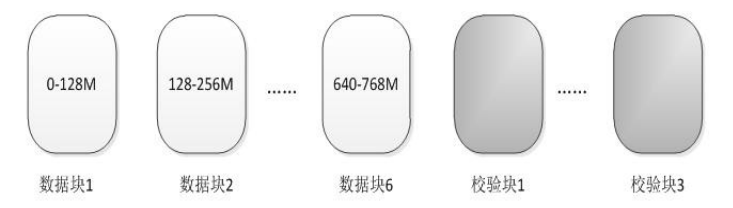
\includegraphics[width=0.9\textwidth]{连续布局示意图.png}
  \caption{连续布局示意图}
\end{figure}

条带布局中,文件会先被切分成一个个大小相等的条带,条带内由若干个相同大小的块构成。文件数据被依次写入条带的各个块中,当一个条带写满之后再写入下一个条带,一个条带的不同块位于不同的存储位置。这种布局能更好地支持小文件的存储,而且不需要缓存较多的数据。如图4.9所示,在用纠删码的方式写入文件时,只需写完一条内6M的数据即可算出校验数据,不需要缓存较多的数据,有利于处理大量小文件,还可以做并行读写操作,提高磁盘的利用率。

\begin{figure}[h]
  \centering
  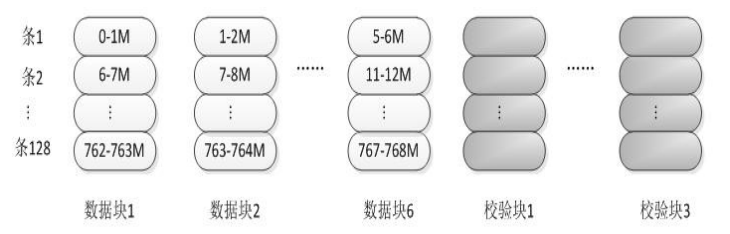
\includegraphics[width=0.9\textwidth]{条形布局示意图.png}
  \caption{条带布局示意图}
\end{figure}

根据以上的分析,我们可知使用条带布局能够更好的实现系统存储大量小文件的目标,因此本系统设计并使用了基于条带分配的文件分配模式。

\subsection{基于条带的文件分配模式}%4.2
由上一节的分析可知,系统为了实现低成本和大量小文件存储的目标,应当使用多副本和纠删码结合的冗余方式,同时使用条带布局来安排文件。本系统设计了基于条带分配的文件分配模式来实现这两项要求,文件的分配模式如图4.10所示,接下来将详细介绍一些相关概念。

\begin{figure}[h]
    \centering
    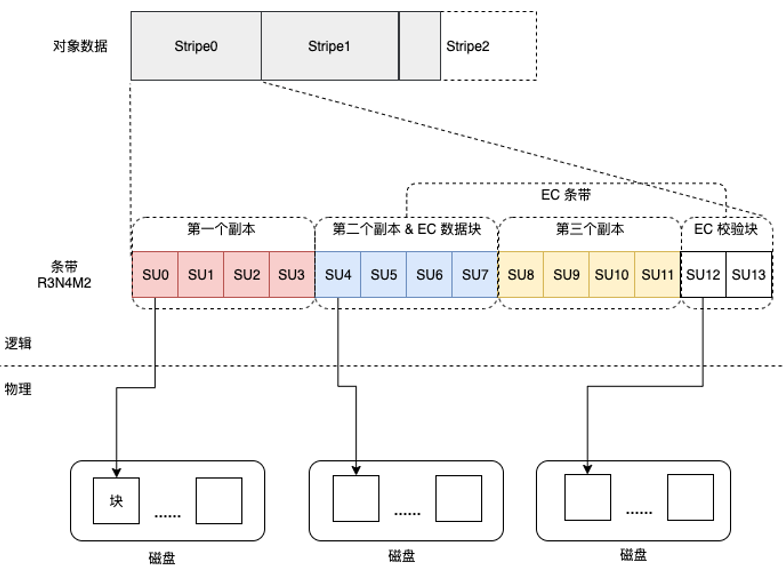
\includegraphics[width=1\textwidth]{文件分配模式示意图.png}
    \caption{文件分配模式示意图}
  \end{figure}

对象数据:系统中用户上传的文件。

块:Block,块是磁盘空间分配的最小单位,块的大小是固定的。块的大小会影响系统中对资源的需求,如果块定的过小,需要维护的块元信息会变多,如果块定的过大,纠删码场景下EC计算需要较多的内存,本系统中定义块的大小为16MB。

块分配模式:系统中的条带需要确定块的分配模式,分配模式有R、N、M三个量需要确定。R代表冗余度,即一份对象数据在条带内有几个副本;N代表一个副本中有几个块;M代表EC校验块的个数,如图4.10所示,图中条带的分配模式是R=3,N=4,M=2则一份对象数据在条带内总共有3个副本,一个副本中有4个块,条带有2个EC校验块。

条带:Stripe,sid表示条带id。条带是在特定块分配模式下分配的多个块的集合,文件以条带的形式保存在系统内,条带内预留了对象数据多副本形式和纠删码形式存储的逻辑空间。数据首先以多副本的形式写入系统,在满足一定条件后,系统会将对象数据编码,得到校验块数据,写入条带内的指定的块上。条带总共需要预留R*N+M个块,多副本形式储存时,需要需要R*N个块,条带数据的校验块数据需要M个校验块,加起来总共为R*N+M个块。

条带单元:StripeUnit(SU),suid表示条带单元id,条带中的每个块称为条带的条带单元。

在这样的文件分配模式下,suid有一定的数学关系:假设条带内块的个数为blockCount,一个块在条带内的位置为blockIndex,那么满足:suid = sid * blockCount + blockIndex。例如在三副本4+2纠删码的分配模式下,如果sid为 0,那么suid的分布如图4.10所示。这个条带有4 * 3 + 2 = 14个块,条带数据的三副本suid为 [0-3]、[4-7]、[8-11],EC校验块suid为 [12-13],对于三副本中的每个块,除了最后一行,前三行每列互为三副本,比如0,4,8互为块的三副本。

基于条带的文件分配模式为了系统的可用性,还考虑数据块的物理存放位置,一个条带中的块不能都放在同一台机器内,否则一台机器出现问题,这个文件都不能进行访问。具体地,以R=3,N=4,M=2的块分配模式为例,设条带的三个副本为S0、S1和S2,每个副本的4个块需要分布在4台不同的机器,且每个块的三副本需要存放在不同机器。当条带内的数据由多副本存储转化为纠删码存储后,假设S1和S2被删除,那么分配的2个校验块需要存放在2台不同的机器上,且这两台机器不能存放S0中的任意块。

本系统设计的条带考虑了多副本存储和纠删码存储的统一,条带根据系统的配置信息切分为若干块,数据初始以多副本的形式写入条带时就会被分成块,经过一段时间条带写满后,多副本数据将会转移为EC数据,而条带内的数据已经以块的形式存在,无需再将数据进行转移分块和计算。也就是说,在进行EC计算时,只需要将冗余的多副本数据从条带中删除,将保留的数据进行EC计算,文件和条带的映射关系保持不变,外部系统不会感知到文件已经由多副本转为了纠删码,这样就避免了额外的读写开销。与此同时,条带内部有一定的数学关系,在读取或写入文件时可以利用条带和块的线性关系来快速定位数据块的位置,能够有效减少元数据系统的存储压力。

\subsection{内部架构设计}%1.3
模块内部使用主从的架构来进行设计,内部逻辑架构如图4.11所示。

master是模块内的主节点,是模块内部的核心服务。它负责管理模块内的条带信息和块信息,分配条带中的块位置,将条带中的块分散到系统的storage中;它也负责管理系统中的所有磁盘信息,接收storage服务定时上报的磁盘信息;它也会和worker服务进行交互,发布任务给worker服务,使其进行EC任务。

storage是模块内负责存储数据的节点,每个storage会管理一台机器上的若干个磁盘,storage在运行时会周期性地向master发送心跳,汇报本节点内存储空间的情况。storage服务不感知条带信息,向storage发起写请求时需要带上块的位置信息。

worker节点负责执行数据的EC任务,它会周期性地从master那里获取条带EC任务,然后和storage交互来执行任务,执行结束后再向master进行汇报。worker服务是一个后台的异步进程,它不直接参与文件的上传下载过程。

除了以上三个实例服务,作为一个存储模块,需要为上层应用提供访问接口。本模块提供了msf代码库供上层应用使用,它封装了模块内部的数据流动细节,上层应用在存取文件时可以不用关心模块内部的情况。msf对外提供文件的写入读取和删除接口,以库的方式部署在项目中,当上层应用需要访问文件存储模块时,可以导入msf的代码,利用msf提供的方法和文件存储模块进行交互。

\begin{figure}[h]
  \centering
  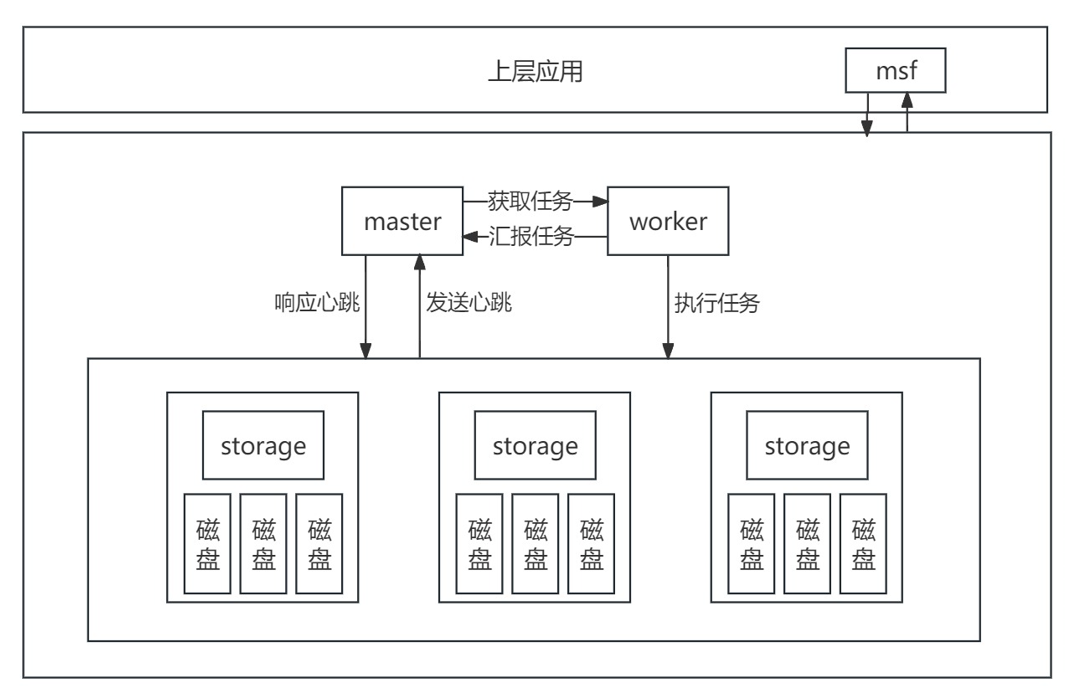
\includegraphics[width=0.95\textwidth]{模块内部逻辑架构图.png}
  \caption{模块内部逻辑架构图}
\end{figure}

接下来的四个小节,将会分别介绍master服务、storage服务、worker服务和msf代码库的概要设计方案。

\subsection{master服务概要设计}

从上一节内部架构设计可知,master服务的主要功能是进行条带管理、磁盘管理和worker服务管理,master服务将会在数据库中保存一些数据并提供一些接口来完成以上功能,接下来将从数据模型和接口说明这两个方面来介绍master服务的概要设计情况。\newline

1. 数据模型

为了实现master的功能,master服务内需要保存一些信息,例如条带信息、条带中块和磁盘的对应关系和磁盘与storage的对应关系等,这些信息并不会保存在元数据服务中,因为这属于存储模块内部的信息,如果由元数据服务来保存的话耦合严重,难以进行系统的扩展。和元数据服务一样,master服务的信息保存在了MongoDB中,同样使用Mongo Sharding来部署,保证了数据的高可用。接下来阐述master的具体数据模型。

(1)条带集合

条带集合保存存储系统内部有多少条带,集合具体内容如表4.6所示。其中mode字段代表条带的分配模式,即R、N、M的值,state字段代表条带的状态,若为0代表条带有空闲容量且可写,值为1代表这个条带已被分配,正在被写入,不能再次被分配,值为2代表条带被写满,等待执行EC任务,值为3代表条带已被写满且已执行完EC任务,冗余块已被删除。

\begin{table}[h]
    \centering
    \caption{条带集合字段表}
    \begin{tabular}{ccc}
      \toprule
      字段   & 字段类型   & 含义                          \\
      \midrule
      sid               & Integer   & 条带id             \\
      mode              & Integer   & 块分配模式          \\
      state             & Integer   & 条带状态            \\
      remainingCapacity & Integer   & 条带剩余可写容量     \\
      \bottomrule
    \end{tabular}
\end{table}

(2)磁盘集合

这个集合保存系统中磁盘的相关信息,具体的数据从heartbeatstorage接口中获取,storage服务会周期性地读取自己管理的磁盘信息,然后通过heartbeatstorage接口向master服务发送心跳,具体的内容如表4.7所示。

\begin{table}[h]
  \centering
  \caption{磁盘集合字段表}
  \begin{tabular}{ccc}
    \toprule
    字段   & 字段类型   & 含义          \\
    \midrule
    diskId     & Integer   & 磁盘id    \\
    host       & String    & ip地址    \\
    totalCount & Integer   & 总块数    \\
    availCount & Integer   & 可用块数  \\
    \bottomrule
  \end{tabular}
\end{table}

(3)块集合

这个集合保存存储系统中块的信息,主要作用是记录条带中的块和磁盘的映射关系,每个块具体落在哪个磁盘中将在这个集合中记录。集合的具体内容如表4.8所示。

\begin{table}[h]
    \centering
    \caption{块集合字段表}
    \begin{tabular}{ccc}
      \toprule
      字段   & 字段类型   & 含义                   \\
      \midrule
      suId     & Integer   & 块id                 \\
      diskId   & Integer   & 磁盘id                \\
      \bottomrule
    \end{tabular}
\end{table}

(4)EC任务集合

EC任务集合保存尚未执行的EC任务,EC任务需要读取多个块的数据,然后经过计算后将得到的数据写到新的块中,EC任务集合中的state字段代表EC任务的状态,值为0代表待执行,值为1代表执行中,hosts字段代表需要参与到EC任务的磁盘的访问地址,disks代表块所存在的磁盘的id。这个集合的具体内容如表4.9所示。

\begin{table}[h]
    \centering
    \caption{EC任务集合字段表}
    \begin{tabular}{ccc}
      \toprule
      字段   & 字段类型   & 含义                          \\
      \midrule
      id     & Integer & EC任务id                 \\
      sid    & Integer & 待EC的条带的id                \\
      mode   & Integer & 块分配模式                 \\
      state  & Integer & EC任务的状态                \\
      hosts  & Array   & 和EC任务相关的磁盘的访问地址  \\
      disks  & Array   & 和EC任务相关的磁盘id         \\
      \bottomrule
    \end{tabular}
\end{table}

2. 接口说明

master服务提供的接口如表4.10所示。以下是这些接口的详细说明。

\begin{table}[h]
  \centering
  \caption{master服务接口表}
  \begin{tabular}{ccp{2.5cm}p{2cm}p{3cm}}
    \toprule
    接口功能   & 请求方式    & 请求路径     & 请求体    & 响应内容                     \\
    \midrule
    接收storage心跳       & POST  & /heartbeatstorage                & storage中磁盘的相关信息   & 磁盘相关信息的反馈\\
    worker获取任务        & GET   & /acquiretask\newline/<maxCount>  & -                        & 任务的详细信息\\
    worker完成任务        & POST  & /completetask                    & 任务的相关信息            & master是否响应成功\\
    分配条带              & GET   & /allocstripes\newline/<size>     & -                        & 分配的条带信息\\
    更新条带信息          & POST  & /updatestripes                   & 条带的信息                & 是否成功更新条带信息\\
    获取条带信息          & GET   & /getstripe\newline/<sId>    & -                        & 条带的详细信息\\
    \bottomrule
  \end{tabular}
\end{table}	

heartbeatstorage:storage服务需要定时向master汇报自己的状态,例如机器上管理了多少个磁盘、每个磁盘的可用容量和剩余容量是多少、磁盘的状态等信息。master用这个接口来接收storage服务上报的信息,在收到心跳后向storage做出响应,表示已经收到storage的信息。

acquiretask:worker在运行过程中会不断的向master获取EC任务,通过这个接口worker可以知道哪些条带已经写满,进而对这些条带进行EC计算。master开放这个接口供worker来获取EC任务。worker可以并行执行任务,因此可以一次性向master获取多个任务,maxCount代表这次请求最多能接收多少个任务。

completetask:woker在执行完EC任务后调用这个接口向master上报,告知这个条带的多副本块已被删除。

allocstripes:在上传文件时,文件需要被写入到条带中,master开放这个接口供上层应用来获取条带,master会根据路径参数中的<size>来得知需要分配多少空间的条带,分配过程中会计算出一个容量零头,产生这个零头的原因是每个条带的可写容量是固定的,但是文件的大小不一定是条带可写容量的整数倍。系统会优先使用最佳适应的策略来寻找已分配的条带去满足零头的需求,最佳适应策略的缺点是产生的碎片比较小,难以利用,但本系统为大量小文件存储进行设计,小文件可以将这些碎片进行填充,使分配出去的块尽量被使用,实现磁盘利用最大化。如果没有条带的剩余空间大于这个零头,master会为这个零头新建一个条带。这个过程可以参考图4.12所示的活动图。

\begin{figure}
  \centering
  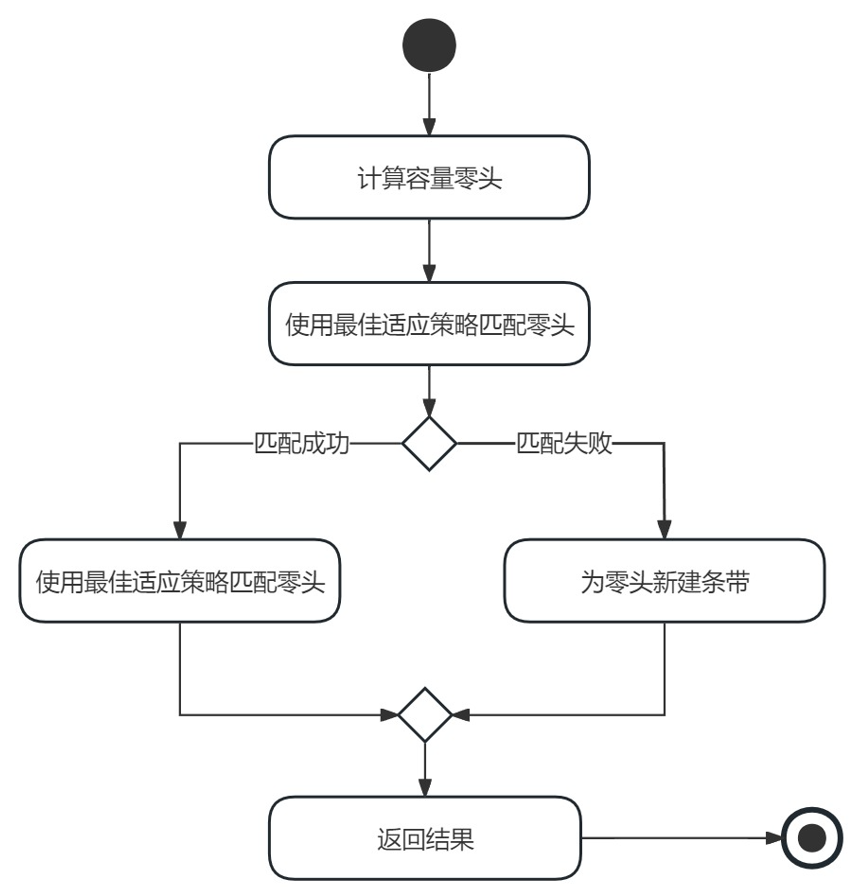
\includegraphics[width=0.59\textwidth]{分配条带活动图.png}
  \caption{allocstripes接口活动图}
\end{figure}

updatestripes:这个接口是master服务用来获知条带信息的接口,条带分配后会被锁定,当条带写完后需要解锁时需要调用这个接口来进行解锁。当某个条带被写满或被删除后,需要通过这个接口告知master条带的新状态,如果有些条带还有剩余空间,也需要通过这个接口告知master条带的剩余空间。

getstripe:这个接口的作用是让msf根据条带id获知条带内的详细信息,当msf需要下载文件时,msf会得到文件是由哪些条带组成的,msf需要调用这个接口,向master获取条带内各个块的信息,最重要的是得知每个块存储在哪个磁盘内和如何访问对应的磁盘,这个时候需要master将块对应的磁盘id返回,同时需要返回访问对应磁盘的ip地址。

通过以上接口,master服务可以和文件存储模块中的各个其他服务进行通信,也可以及时地了解其他模块的状态,对其他模块做出相关的控制。

master服务作为文件存储模块中的重要服务,需要保证它的可用性,由于数据都保存在了MongoDB中,master可以被视为无状态的服务,只需要在系统中启动多个master服务,单个master服务不能正常提供服务时,系统中master服务依然可以由冗余部署的master持续提供服务。

\subsection{storage服务概要设计}

1. 磁盘划分方案

storage以块为单位进行数据的读写,为了提升系统的读写效率,本系统在向磁盘写入文件时没有使用操作系统的文件作为数据的载体,而是直接将数据存入磁盘中。接下来详细介绍storage是如何划分磁盘的。

\begin{figure}
  \centering
  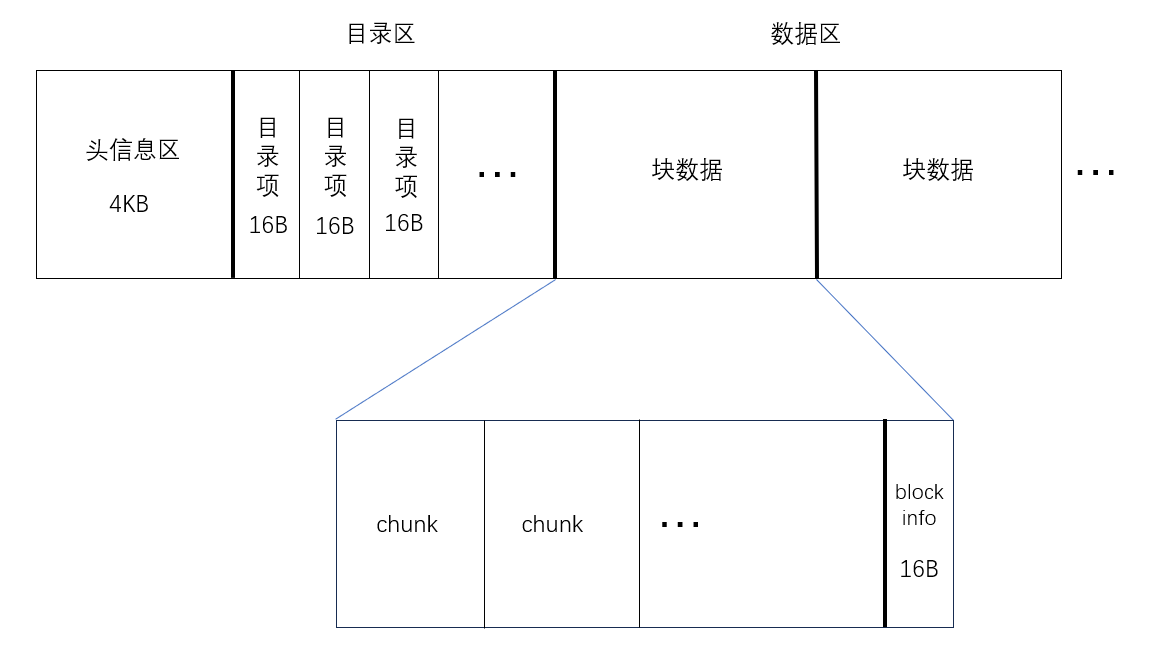
\includegraphics[width=0.85\textwidth]{磁盘划分示意图.png}
  \caption{磁盘划分示意图}
\end{figure}

storage将磁盘划分为头信息区(Header)、目录区(Directory)和数据区(Blocks)这三类区域,它们的分布如图4.13所示,下面给出每个区域存储的内容和大小。

(1)头信息区:头信息区的大小是4KB,原因是对于固态硬盘来说,存取的最小单位是4096个字节,而磁盘头信息的内容很少进行改动,我们希望尽量少地读取这部分信息,因此把它放在单独的一个扇区内,避免读写其他数据时多次访问这部分数据,造成额外的开销。头信息区中需要保存以下内容:

Tag:大小4字节,是固定的标记位,用来表示磁盘已被初始化

DiskID:大小4字节,用来表示磁盘的ID号

BlockCount:大小4字节,用来表示磁盘中数据块的总数

BlockSize:大小4字节,用来表示磁盘中每个数据块的大小

ChunkSize:大小4字节,用来表示数据片的大小

Reserved:这是保留空间,用来填补不足4KB的部分

CRC32:大小4字节,用来保存Header前4K-4字节的32位循环冗余校验码的值

(2)目录区:目录区保存的是每个块的元信息,每个块的元信息一个目录项来保存,这一部分的内容也不会经常改变,一个目录项的大小为16字节,每个目录项具体有以内容:

SuId:大小8字节,用来表示块的ID号

DeleteTime:大小4字节,用来表示块删除的时间

CRC32:大小4字节,是目录项中前12字节的32位循环冗余校验码的值

(3)数据区:数据区保存的是块的具体数据内容,每个块的数据由若干个数据片(Chunk)和一个块信息(BlockInfo)组成。

数据片是最小的数据读写单位,一个数据片的大小被称为ChunkSize,ChunkSize的大小是固定的,数据片的前四个字节是后面ChunkSize-4字节的crc32校验和,读取数据时需要将整个数据片读出以校验数据的正确性。写数据时最优一次写一个或多个完整的数据片到磁盘,如果写的数据片大小不满ChunkSize,也需要生成校验和将数据写入磁盘,因此在一个块中,除了最后一个正在写入的数据片,前面的数据片大小都是ChunkSize。ChunkSize如果定的过大,在小文件的场景会有读放大(必须读出整个Chunk),如果ChunkSize定的过小,Chunk中的校验和占用空间会变多,本系统将ChunkSize定为64KB。

相较于目录项,BlockInfo保存了块数据中经常变动的元信息,这样做的目的是为了提高写入性能,假设所有块的元信息都存储在目录区,那么每次写Chunk都需要更新目录区中的块大小,在机械盘中,由于块数据离目录区比较远,会产生较大的磁盘寻址延迟,因此需要把这部分可能频繁修改的元数据放在块数据的尾部,减少磁盘寻址延迟,BlockInfo具体保存的信息如下所示:

SuId:大小8字节,用来表示块ID

DataLen:大小4字节,代表这个块中存储的数据大小

InfoCRC3:大小4字节,是BlockInfo中前12字节的32位循环冗余校验码的值

2. 接口说明

\begin{table}[h]
    \centering
    \caption{storage服务接口表}
    \begin{tabular}{ccp{4cm}p{2cm}p{3cm}}
      \toprule
      接口功能   & 请求方式    & 请求路径     & 请求体    & 响应内容                     \\
      \midrule
      上传数据      & POST   & /putat/<diskId>/<suid>\newline/<offset>/<size> & 数据内容      & 是否上传成功\\
      下载数据      & GET    & /get/<diskId>\newline/<suid>/<offset>/<size>   & -            & 所需的数据\\
      删除块        & DELETE & /delete/<diskId>/<suid>                        & -            & 是否删除成功\\
      分配块        & POST   & /allocateblock                                 & 分配的块信息  & 是否分配成功\\
      释放块        & POST   & /freeblock                                     & 释放的块信息  & 是否释放成功\\
      \bottomrule
    \end{tabular}
\end{table}	

为了向master汇报本机的磁盘信息,storage服务启动后会定时调用master服务的heartbeatstorage接口上报所管理的磁盘信息。与此同时,storage服务也需要暴露一些接口,以供其他应用来访问磁盘中的数据,这些接口如表4.11所示。

请求路径中<diskId>代表磁盘的id,<suid>代表块号,<offset>代表块内偏移量,<size>代表数据的大小。通过上传数据、下载数据和删除块这三个接口,外部服务可以访问系统中实际存储数据的磁盘,从而实现对数据的操作。分配块接口是为master划分条带服务的,当master需要使用磁盘上的某个空闲块时,会向调用storage的分配块接口,告知storage某个磁盘上的空闲块即将被使用,应将这个空闲的状态改为使用中,同理,当需要释放的时候需要调用释放块接口来将已分配的块进行释放。

\subsection{worker服务概要设计}
worker服务可以在master服务开始运行后,由master负责启动woker。worker服务的任务是执行EC任务,把已经写满的条带进行EC计算,然后将条带中多副本部分的冗余块进行删除,运行过程如图4.14所示。

\begin{figure}[h]
  \centering
  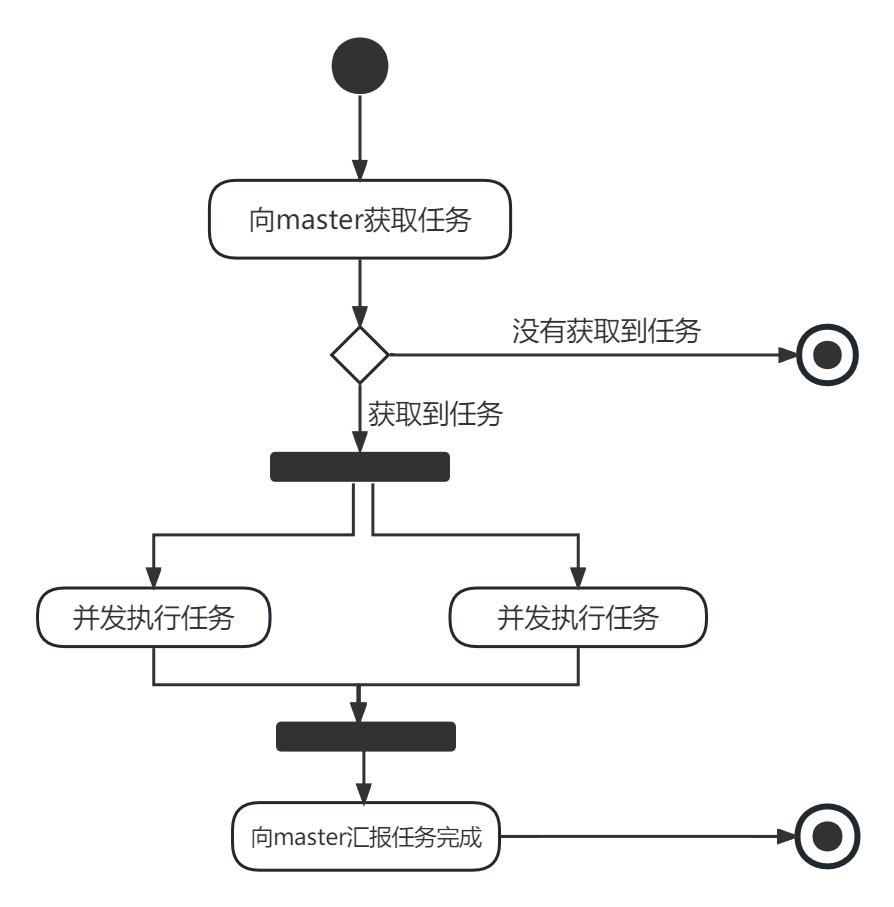
\includegraphics[width=0.6\textwidth]{worker活动图.png}
  \caption{worker任务活动图}
\end{figure}

worker可以一次从master中批量获取任务,然后并发地执行EC任务,加速EC的过程。

\subsection{msf库概要设计}

msf对外提供对象的写入读取和删除的方法,上层应用中的代码会直接调用msf的方法来去进行文件数据的操作。这样做的好处是将上层应用和文件存储模块进行解耦,上层应用无需知道文件存储模块的实现细节,只需调用msf中的方法即可完成操作。msf需要提供以下三种方法,如表4.12所示。

\begin{table}[h]
  \centering
  \caption{msf服务方法表}
  \begin{tabular}{cccc}
    \toprule
    方法功能   & 方法名    & 参数     & 返回值               \\
    \midrule
    下载数据      & get    & fileHandle、fmd5  & data       \\
    \addlinespace
    上传数据      & put    & data              & fileHandle \\
    \addlinespace
    删除数据      & delete & fileHandle        & result     \\
    \bottomrule
  \end{tabular}
\end{table}	

get方法需要上层应用从元数据数据库中获得文件的fileHandle,msf得到fileHandle后到master服务中解析条带信息就知道文件具体存储在哪些storage的哪些磁盘上,根据这些信息msf会访问storage读取块数据,全部数据读取完毕后会计算得到文件的md5是否和参数中的md5一致,如果不一致则代表数据出现异常,需要利用冗余信息重新读取文件,以返回正确的数据。

put方法负责文件的上传,msf得到需要上传的数据后,会向master申请条带,并将数据写入到条带对应的块中,然后会将fileHandle返回。返回的fileHandle代表文件在文件存储模块的位置,上传应用需要将fileHandle信息记录到元数据数据库中。

delete方法需要上传应用提供文件的fileHandle,然后根据fileHandle提供的信息将对应的块进行删除,同时还要告知master条带的变动情况。

\section{本章小节}
本章首先进行了系统整体架构的介绍,系统使用了分层的架构来进行设计。然后介绍了四个功能模块的概要设计,给出了每个功能实现的大致流程。接下来进行元数据模块的概要设计,介绍了元数据数据库的选型以及系统的数据模型。最后进行了文件存储模块的概要设计,对它的进行分析并给出内部架构的设计,然后介绍了文件存储模块内部每个服务的设计方案。